%!TEX encoding = UTF-8 Unicode  
\documentclass{ZJUthesis}
\usepackage[top=1in, bottom=1in, left=1.25in, right=1.25in]{geometry}   % 调整页边距
\usepackage{amssymb}
\setcounter{tocdepth}{3}
\usepackage{graphicx}
\usepackage{url}
\usepackage{colortbl}
\usepackage{amsmath,epsfig,amssymb}
\usepackage{amsfonts,amssymb}%,pxfonts}%txfonts}%,pxfonts}
\usepackage{subfig}
\usepackage{makeidx}  % allows for indexgeneration
\usepackage{url}
\usepackage{pst-node}
\usepackage{pstricks}
\usepackage{pstricks-add}
\usepackage{booktabs}
\usepackage{overpic}
\usepackage{caption}
\usepackage{textcomp}
\usepackage{multirow}
\usepackage{marvosym}  % 画笑脸用的
\usepackage{pdfpages}

 \usepackage{clrscode}
\usepackage{listings}

\lstset{language=C++}%这条命令可以让LaTeX排版时将C++键字突出显示
\usepackage{enumerate}

\lstset{breaklines}%这条命令可以让LaTeX自动将长的代码行换行排版

\lstset{extendedchars=false}%这一条命令可以解决代码跨页时,章节标题,页眉等汉字不显示的问题


\begin{document}



% 章节标题左对齐
\CTEXsetup[beforeskip={-5ex}, format={\bf\zihao{3}\flushleft}]{chapter}
\CTEXsetup[beforeskip={-5ex}, format={\bf\zihao{-3}\flushleft}]{section}
\CTEXsetup[beforeskip={-5ex}, format={\bf\zihao{-3}\flushleft}]{subsection}


%%%%%%%%%%%%%%%%%%%%%%%%%%%%%%
%% 封面部分
%%%%%%%%%%%%%%%%%%%%%%%%%%%%%%

% 中文封面内容

  \title{稀疏矩阵存储的C++实现}
  \author{唐周若愚 \quad 3110104942}
  \supervisor{王何宇 \quad 副教授}
  \major{信息与计算科学 \quad 2011级}
  \institute{数学系}


  % 诚信承诺书
  \classes{信息与计算科学1102}
  \studentid{3110104942}
  \signitureyear{2015}
  \signituremonth{5}
  \signitureday{26}

  % 封面
  \maketitle

  % 诚信承诺书
  \makeenglishtitle


\includepdf[addtotoc={1,section,1,title in toc,cc},pages=2-2,offset=0cm 0.5cm]{tt.pdf}
%%%%%%%%%%%%%%%%%%%%%%%%%%%%%%
%% 前言部分
%%%%%%%%%%%%%%%%%%%%%%%%%%%%%%
%%\frontmatter





  % 摘要
  %!TEX encoding = UTF-8 Unicode  
\begin{abstract}
在现代的科学计算与工程中,由于经常会对大规模甚至是超大规模的矩阵进行运算,传统的全矩阵运算已经无法满足实际的需求。为了能对这些矩阵进行数值运算,利用矩阵的稀疏性的稀疏矩阵便被创造了出来,大大地缩减了计算的复杂度。而本文则是旨在建立一个底层的稀疏矩阵存储与计算的C++库,供计算使用者使用,方便快捷地实现稀疏矩阵的运算而无需顾及稀疏矩阵的底层存储。

\keywords{稀疏矩阵、C++、存储}
\end{abstract}


\begin{englishabstract}
In modern scientific computation and industrial projects, the traditional dense matrix cannot satisfy the increasing requirement of calculating large scale matrixes. In order to be able to calculate such matrixes, sparse matrix is created by taking advantage of the sparsity. The complexity of calculating is reduced in a large amount by using sparse matrix. The purpose of this paper is to create a C++ library to storage the sparse matrix for programmers who want to use sparse matrix. With this library, programmers can calculate sparse matrix easily and quickly without thinkink about the storage of the sparse matrix.

\englishkeywords{Sparse Matrix;C++;Storage}
\end{englishabstract}

  % 目录
  \tableofcontents

%%%%%%%%%%%%%%%%%%%%%%%%%%%%%%
%% 正文部分
%%%%%%%%%%%%%%%%%%%%%%%%%%%%%%
%%\mainmatter
  %!TEX encoding = UTF-8 Unicode  
\chapter{引言}
 在实际工程计算中,尤其是在微分方程数值解、线性规划等的有限元分析中,经常出现高阶的矩阵运算,经常出现百万阶、千万阶的矩阵运算,而如果使用全矩阵运算,假设是百万阶的float类型的矩阵,则需要$4*10^{12}B$来存储,也就是4TB的空间,这显然是无法被微型计算机甚至是工作站所接受的。但是通常这些矩阵具有稀疏的性质,拥有着大量的零元,而且通常阶数越高稀疏度越高。这就可以在相当大的程度上减少了存储对于硬件的压力。同时,在计算中,大量对于0的运算是无谓的消耗资源的操作,也可以利用稀疏矩阵来避免这些无谓的操作。而在本研究中编写的稀疏矩阵库可以用来方便快捷的实现稀疏矩阵的存储以及一些基本运算,避免了使用者大量编写存储底层的代码,提高开发效率。


\chapter{研究背景综述}
近年来,在工程应用中,求解高阶矩阵的需求日益增长,全矩阵运算脱离了实际的硬件限制,为了满足这一日益增长的需求,同时这些矩阵通常都有着一个特征——非零元远少于零元,稀疏矩阵这门学科便应运而生。
在 20 世纪 60 年代研发电子网络的电子工程师们是最早的去利用稀疏性来应用稀疏矩阵进行工程上的计算的。
\cite{YousefSaad2003applied}

而在微分方程数值解、线性规划等的有限元分析中,经常出现求解高阶稀疏线性方程组,如利用全矩阵进行存储,则需要$n^2$的空间复杂度和$n^3$的乘法运算时间复杂度,显然,这种程度的运算量是无法被微型计算机,甚至是工作站所接受的。
而利用矩阵的稀疏性,可以有效地减小消耗很多无谓的存储空间以及无谓的计算,在很大的程度上降低了时间和空间复杂度,降低了计算对硬件的需求,使计算成为可能。


\section{稀疏矩阵的定义}
稀疏矩阵是非零元远小于矩阵元素总数,且非零元分布没有规律的矩阵。
\cite{YousefSaad2003applied}

\section{稀疏矩阵已有存储方式}
在这些年的发展中,出现了很多的存储方法,比如:对角线存贮法、对称矩阵的变带宽存贮法、坐标存贮法、Elipack-Itpack存贮法、CSR存贮法、Shermans存贮法、超矩阵存贮法、动态存贮方案等。\cite{sparseMatrixTech2006Zhangsun}

\subsection{三元组(Triplet)存储}
顾名思义,三元组存储方法就是分别存储矩阵的非零元所在的行列索引值,以及与之对应的非零元的值的存储方案。\cite{fengguangxiang2010.}
\newline
三元组存储方案有着直观、易于实现、顺序无关的特性,但是与传统的存储方法一样,三元组存储方案不便于求解算法的使用,不利于利用矩阵的稀疏性。
典型的C语言实现为\newline
\begin{lstlisting}

struct triplet_matrix{ 
	int *Ti;/*row pointer*/ 
	int *Tj;/*column pointer*/
	double *Tx;/*value pointer*/
	int Tnz;/*number of entries*/
	int Tnrow;/*number of rows*/
	int Tncol;/*number of columns*/
};

\end{lstlisting}
下面对应于矩阵的三元组存储:
\newline\newline\newline\newline\newline
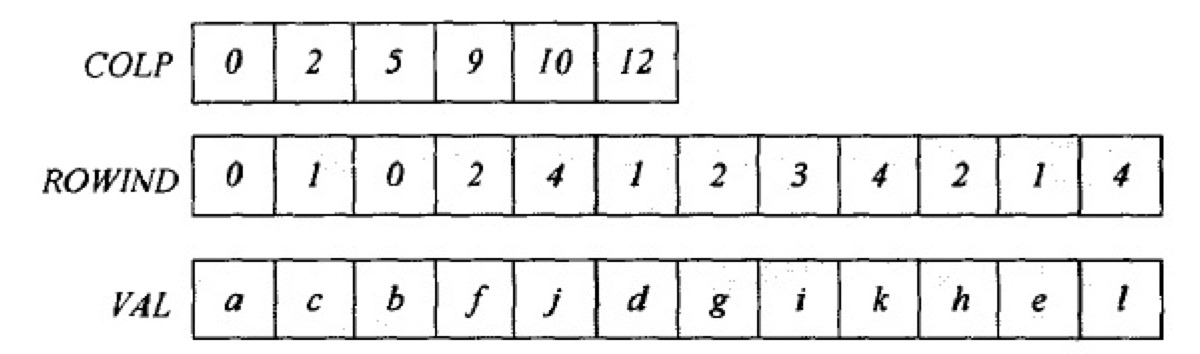
\includegraphics[scale=0.25]{triplet.png}

\subsection{十字链表(Orthogonal List)存储}
稀疏矩阵可以用上述的三元组存储方式存储,但是当稀疏矩阵的非零元的位置或个数经常变化时,使用三元组存储方式就效率低下,而十字链表法能有效的提高存取效率。十字链表法不仅为稀疏矩阵的每一行设置一个单独的行循环链表,而且同样为每一列设置一个单独的列循环链表。因此,每一个非零元同时存在于两个链表中,即包含它们的行循环链表和列循环链表,亦即这两个链表的交汇处。\newline
稀疏矩阵的链表节点需要同时存储所在的行号(row)、列号(col)、相应的元素值(value)、向下指针(down)、向右指针(right)。典型的C语言结构实现为:
\begin{lstlisting}
typedef struct node {
    int row, col;
    union {
        int val;
        struct node *ptr;
    };             //value域包括两种类型
    struct node *right, *down;
}CNode, *CrossLink;
\end{lstlisting}
\subsection{列压缩CSS(Compressed-column storage)存储}
任何矩阵的运算都涉及到矩阵的存储与读取操作,因此,存取效率对于矩阵运算的效率有着极大的影响。\newline
许多开源库采用了该存储结构,如UMFPACK、TAUCS等。列压缩存储方案较前面的三元组存储方案较不好理解,但是在矩阵计算中能更为高效地利用矩阵的稀疏性,而这也就是各大求解器采用这一存储方案的原因。\cite{fengguangxiang2010.}
\newline
列压缩存储维护了三组数据——(各列非零元的累加值,按递增的顺序存储的每列的非零元的行索引值,对应第二组数据行索引值位置对应的非零元的值)。
典型的C语言结构实现为\newline
\begin{lstlisting}

struct cc_matrix{ 
	int *Ai;/*row index*/ 
	int *Ap;/*length ncol+1*/
	double *Ax;
	
	int Ancol;
	int Anrow;
};

\end{lstlisting}
下面对应于矩阵的列压缩存储:
\newline\newline\newline\newline\newline
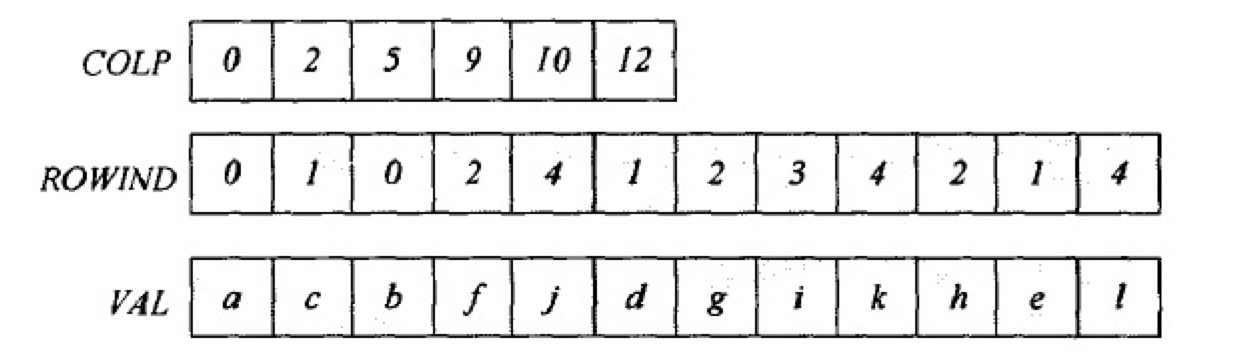
\includegraphics[scale=0.25]{ccmatrix.png}

\subsection{行压缩存储方式(Compressed Row Storage)}

CRS存储可以高效地存取任意一行非零元素,但存取任意一列非零元则需要遍历整个CRS存储结构。相应地,与CRS存储的稀疏矩阵相关的算法要高效的编程实现,算法的计算顺序必须按行来进行。\cite{fengguangxiang2010.}
下面对应于CRS存储:
\newline\newline\newline

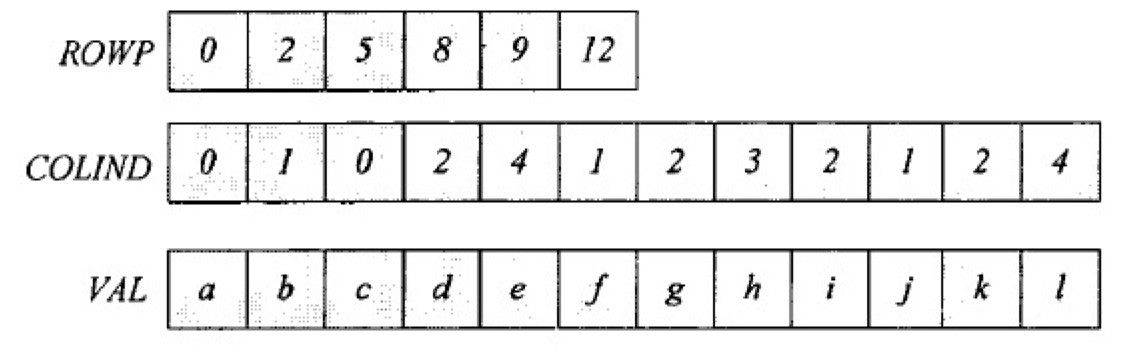
\includegraphics[scale=0.25]{crs.png}
\newline\newline
我们可以发现,ROWP数组存储的时行非零元的增长量。COLIND则存储的是列索引值,典型的C语言结构实现为\newline

\begin{lstlisting}

struct cr_matrix{ 
	int *Ri;/*col index*/ 
	int *Rp;/*length nrow+1*/ 
	double *Rx; 
	int Rncol;
	int Rnrow;
};

\end{lstlisting}

显然,越是简单的数据结构,存取操作的效率越高,亦即寻址操作的效率越高。例如,传统的稠密矩阵的存储方案只需根据行列索引值即可计算得到数据所在的地址,轻松高效的实现存取操作。在列压缩存储的稀疏矩阵中,显然能高效地存取矩阵的一列,但是,存取行的效率是极为低下的。因此,在矩阵的运算中,我们希望能尽可能地按列进行,而不是按行进行。CRS存储可以高效地存取任意一行非零元素,但存取任意一列非零元则需要遍历整个CRS存储结构。相应地,与CRS存储的稀疏矩阵相关的算法要高效的编程实现,算法的计算顺序必须按行来进行。\cite{fengguangxiang2010.}
下面对应于CRS存储:
\newline\newline\newline

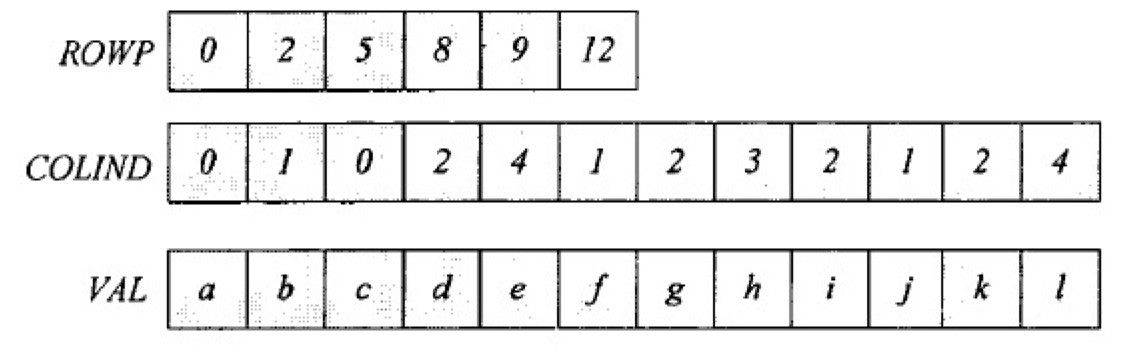
\includegraphics[scale=0.25]{crs.png}
\newline\newline
我们可以发现,ROWP数组存储的时行非零元的增长量。COLIND则存储的是列索引值,典型的C语言结构实现为\newline

\begin{lstlisting}

struct cr_matrix{ 
	int *Ri;/*col index*/ 
	int *Rp;/*length nrow+1*/ 
	double *Rx; 
	int Rncol;
	int Rnrow;
};

\end{lstlisting}

显然,越是简单的数据结构,存取操作的效率越高,亦即寻址操作的效率越高。例如,传统的稠密矩阵的存储方案只需根据行列索引值即可计算得到数据所在的地址,轻松高效的实现存取操作。在列压缩存储的稀疏矩阵中,显然能高效地存取矩阵的一列,但是,存取行的效率是极为低下的。因此,在矩阵的运算中,我们希望能尽可能地按列进行,而不是按行进行。

\section{已有的处理稀疏矩阵存储与运算的开源库}

在做稀疏矩阵的计算时,通常都是做一系列的基本运算,如:矩阵转置、矩阵向量乘法、矩阵矩阵乘法、数乘等。为了能得到更好的效率,许多研究者致力于寻找对于这些计算最优的存储结构及计算算法,同时提供了许多类库供科学计算使用,如:Portable, ExtensibleToolkit for Scientific Computation(PETSc)、Boost、GNU Scientific Library (GSL)等。\newline
例如,在Boost-uBLAS中有着稀疏矩阵的模板mapped\_matrix<T, F, A>(元素映射矩阵存储形式)、compressed\_matrix<T, F, IB, IA, TA>(压缩存储格式)、coordinat\_matrix<T, F, IB, IA, TA>(坐标存储格式)。
分别有着如下示例:\cite{boost_ublas}\newline
\textbf{mapped\_matrix:}
\begin{lstlisting}

#include <boost/numeric/ublas/matrix_sparse.hpp>
#include <boost/numeric/ublas/io.hpp>

int main () {
    using namespace boost::numeric::ublas;
    mapped_matrix<double> m (3, 3, 3 * 3);
    for (unsigned i = 0; i < m.size1 (); ++ i)
        for (unsigned j = 0; j < m.size2 (); ++ j)
            m (i, j) = 3 * i + j;
    std::cout << m << std::endl;
}

\end{lstlisting}

\textbf{compressed\_matrix:}
\begin{lstlisting}

#include <boost/numeric/ublas/matrix_sparse.hpp>
#include <boost/numeric/ublas/io.hpp>

int main () {
    using namespace boost::numeric::ublas;
    compressed_matrix<double> m (3, 3, 3 * 3);
    for (unsigned i = 0; i < m.size1 (); ++ i)
        for (unsigned j = 0; j < m.size2 (); ++ j)
            m (i, j) = 3 * i + j;
    std::cout << m << std::endl;
}

\end{lstlisting}

\textbf{coordinate\_matrix:}
\begin{lstlisting}

#include <boost/numeric/ublas/matrix_sparse.hpp>
#include <boost/numeric/ublas/io.hpp>

int main () {
    using namespace boost::numeric::ublas;
    coordinate_matrix<double> m (3, 3, 3 * 3);
    for (unsigned i = 0; i < m.size1 (); ++ i)
        for (unsigned j = 0; j < m.size2 (); ++ j)
            m (i, j) = 3 * i + j;
    std::cout << m << std::endl;
}
\end{lstlisting}

\section{稀疏矩阵的数乘}
根据数乘的定义,若矩阵A的=\{$a_{ij}$\},则kA=\{$ka_{ij}$\},则稀疏矩阵的数乘可以简单的定义为所有非零元乘上这个数。例如:对(1)实现的三元组存储的稀疏矩阵的数乘可以用如下函数进行计算:
\begin{lstlisting}
void multi(triplet_matrix matrix,double k){
	for(int i=0;i<Tnz;i++){
		*Tx[i]=*Tx[i]*k;
	}
}
\end{lstlisting}

\section{稀疏矩阵的矩阵向量乘法}
根据矩阵向量乘法的定义:
$$
\left (                 
\begin{array}{cccc}   
    a_{11} & a_{12}& \cdots & a_{1n}\\  
    a_{21} & a_{22}& \cdots & a_{2n}\\  
     \vdots & \vdots& \ddots  & \vdots \\ 
    a_{n1} & a_{n2}& \cdots & a_{nn}\\     
\end{array}
\right)          
\left (                 
\begin{array}{c}   
    b_{1} \\  
    b_{2} \\  
    \vdots \\  
    b_{n} \\  
\end{array}
\right)           
=
\left (                 
\begin{array}{c}   
    a_{11}b_{1}+ a_{12}b_{2}+\cdots+a_{1n}b_{n}\\  
    a_{21}b_{1}+ a_{22}b_{2}+\cdots+a_{2n}b_{n}\\  
    \vdots \\  
     a_{n1}b_{1}+ a_{n2}b_{2}+\cdots+a_{nn}b_{n}\\  
\end{array}
\right)   
$$
由于零元参与运算对计算结果没有影响,所以在计算中可以不对零元计算,亦即在稀疏矩阵的矩阵向量运算中,可以只对非零元进行计算。亦即对A的每一列j的非零元$a_{ij}$执行
$$z_i=y_i+a_{ij}x_j$$

那么,我们可以很方便的利用矩阵的稀疏性对列压缩存储的稀疏矩阵进行上述操作,示例代码如下
\begin{lstlisting}
for(int j=0;j<Ancol;j++){
	for(int p=Ap[j];p<Ap[j+1];p++){
		z[Ai[p]]=Ax[p]*x[j]+y[Ai[p]];
	}
}
\end{lstlisting}



\section{稀疏矩阵的矩阵矩阵乘法}
根据矩阵向量乘法的定义:
$$
\left (                 
\begin{array}{cccc}   
    a_{11} & a_{12}& \cdots & a_{1n}\\  
    a_{21} & a_{22}& \cdots & a_{2n}\\  
     \vdots & \vdots& \ddots  & \vdots \\ 
    a_{n1} & a_{n2}& \cdots & a_{nn}\\     
\end{array}
\right)          
\left (                 
\begin{array}{cccc}   
     b_{11} & b_{12}& \cdots & b_{1n}\\  
    b_{21} & b_{22}& \cdots & b_{2n}\\  
     \vdots & \vdots& \ddots  & \vdots \\ 
    b_{n1} & b_{n2}& \cdots & b_{nn}\\ 
    \end{array}
\right)           
=
\left (                 
\begin{array}{cccc}   
     c_{11} & c_{12}& \cdots & c_{1n}\\  
    c_{21} & c_{22}& \cdots & c_{2n}\\  
     \vdots & \vdots& \ddots  & \vdots and\\ 
    c_{n1} & c_{n2}& \cdots & c_{nn}\\ 
\end{array}
\right)   
$$
其中,对于任意的i,j,有$$
c_{ij}=\sum_{k=1}^na_{ik}b_{kj}
$$
由于零元参与运算无意义,在计算中可以将零元不进行运算。
亦即$$
c_{ij}=\sum_{k=1,a_{ik}\neq 0,b_{kj} \neq 0}^na_{ik}b_{kj}
$$


  %!TEX encoding = UTF-8 Unicode  
\chapter{研究的目标、内容及研究方法}
\section{研究的目标}
利用c++语言在linux平台下的g++编译器上编写一个库,实现稀疏矩阵的行压缩存储方式(Compressed Row Storage)存储,并可以实现并行计算稀疏矩阵的矩阵乘法、数乘等运算,可以在实际的科学计算中进行使用。
 \section{研究内容}
  在linux平台下,基于g++编译器、C++标准库,编写稀疏矩阵存储的C++库,实现稀疏矩阵的行压缩存储方式(Compressed Row Storage),同时实现一些稀疏矩阵的基本运算,如矩阵乘法、数乘等。而为了更好地发挥现代多核心CPU的性能,需要实现多线程并行计算,为以后可能进行的集群运算留下可以使用的接口。
  
  \section{研究方法}
  实现稀疏矩阵的行压缩存储方式(Compressed Row Storage),通过数组存储非零元的增长量、列索引值和非零元值来实现稀疏矩阵的存储。为了实现可变长数组的存储,利用C++的STL中的vector来存储数据。
  
  具体实现数据结构如下:
  \begin{lstlisting}

class sparseMatrix
{
private:
    int n_col;		/**< number of the columns. */
    int n_row;		/**< number of the rows. */
    int n_couple;
public:
    std::vector<double> ele; /**< the array to story the values of the elements. */
    std::vector<int> col;	/**< the column  index of the non-zero elements. */
    std::vector<int> row;	/**< the row index of the non-zero elements. */
}
\end{lstlisting}

而为了更好地利用现代多核心CPU的性能,利用thread库实现多线程并行计算,更为有效地利用CPU的并行性能,为未来用于集群计算留下可以使用的接口。而在并行计算中,由于存在多个线程同时操作某一块内存,出现“脏数据”的情况,为了防止多线程并行计算中“脏数据”的出现,利用mutex互斥锁保障进程安全性,将正在运算的内存进行加锁,防止被另一线程同时操作,在操作完成后,进行解锁,供另一线程操作。而在不同的机型上,由于硬件配置、软件配置不一,最优线程数也不一,为了实现更好的利用计算机硬件性能,利用C++的预定义来由程序编写者自行设定线程数。
\newline
由于在实际工程中,经常遇到的矩阵操作有矩阵数乘运算、矩阵矩阵乘法、矩阵向量乘法等等,需要实现稀疏矩阵的一些基本运算(矩阵数乘运算、矩阵矩阵乘法、矩阵向量乘法等)。而为了实现稀疏矩阵的矩阵矩阵乘法和矩阵向量乘法,可以参考全矩阵矩阵矩阵乘法和矩阵向量乘法算法,利用稀疏矩阵的零元不参与计算的特性,按照稀疏矩阵存储的结构,较全矩阵计算省略大量计算,实现稀疏矩阵计算的优势——更为高效的计算。

  \chapter{实验结果}
  在iMac 5k平台上进行测试(3.5 GHz Intel Core i5,8 GB 1600 MHz DDR3),分别测试sparseMatrix和boost-ublas,测试代码如下:
  
  \textbf{使用sparseMatrix.h}
  \begin{lstlisting}

#include <iostream>
#include "sparseMatrix.h"
#include<stdlib.h>
#include "complexSparseMatrix.h"

#define ROW 100000 //行数
#define COL 100000 //列数
#define COUPLE 1500   //每行最多非零数
#define NONE_ZERO_PERCENT 0.01


int main(int argc, const char * argv[]) {
    //初始化稀疏矩阵
    sparseMatrix* sparse=new sparseMatrix(ROW,COL,COUPLE);
    sparse->init(NONE_ZERO_PERCENT);
    sparse->compress();
  
    clock_t start,finish;double duration;
    start=clock();
    multi(sparse, sparse);
    finish=clock();
    duration=1000*(double)(finish-start)/CLOCKS_PER_SEC;
    std::cout<<duration<<std::endl;
    
    multi(sparse, sparse)->show('B');
    
    return 0;
}


\end{lstlisting}
\textbf{使用boost\_ublas}
\begin{lstlisting}
  #include <iostream>
#include<fstream>
#include "boost/numeric/ublas/matrix_sparse.hpp"
#include "boost/numeric/ublas/io.hpp"
using namespace std;
int main ( ) {
    using namespace boost::numeric::ublas ;
    compressed_matrix <double> m ( 10000 , 1000) ;
    
    ifstream infile;
    infile.open("/Users/tzry/Desktop/graduation-project/sparse/output.txt");
    
    while (infile.good()&&!infile.eof()) {
        int i,j;
        double v;
        infile>>i>>j>>v;
        m(i-1,j-1)=v;
        
    }
    
    
    clock_t start,finish;double duration;
    start=clock();

    m=boost::numeric::ublas::prod(m,m);
    
    finish=clock();
    duration=1000*(double)(finish-start)/CLOCKS_PER_SEC;
    std::cout<<duration<<std::endl;

}
\end{lstlisting}
 测试结果如下:

\begin{tabular}{|c|c|c|c|}
\hline \multicolumn{4}{|c|}{10000阶稀疏度为0.01的稀疏矩阵的矩阵矩阵乘法}\\
\hline 单行最大非零元个数&200&500&1000\\
\hline sparseMatrix&85404.1ms&85129.4ms&87244.9ms\\
\hline boost$\_$ublas&43823.6ms&330923ms&1.470550e+06ms\\
\hline
\end{tabular}



\chapter{结论}
根据本文第四部分内容,boost$\_$ublas库的效率在很大程度上取决于输入参数的好坏,而sparseMatrix则效率与输入参数的好坏相关系数很小。虽然在好的参数条件下,boost$\_$ublas的效率更高,但是,sparseMatrix的鲁棒性更好,不容易受到差的输入参数的影响。sparseMatrix在较差的参数条件下与较好地参数条件下,效率基本没有区别。
\newline
在实际计算中,遇到不容易知道参数如何选择,或者每行的非零元数量经常变化,且变化较大时,使用sparseMatrix库能有效地提高使用效率。









  % 附录
  \appendix
  %!TEX encoding = UTF-8 Unicode  
\chapter{sparseMatrix库}

\section{sparseMatrix.h}
\begin{lstlisting}

#ifndef sparseMatrix_h
#define sparseMatrix_h
#include <vector>
#include <iostream>
#include <fstream>
#include "tmpSparse.h"
#include<thread>
#include"sparseVector.h"

#define THREADCOUNT 1//线程数




class sparseMatrix
{
private:
    int n_col;		/**< number of the columns. */
    int n_row;		/**< number of the rows. */
    int n_couple;
    
    
    std::mutex m;//互斥量
    
public:
    
    int missionRow=0;
    
    std::vector<double> ele; /**< the array to story the values of the elements. */
    std::vector<int> col;	/**< the column  index of the non-zero elements. */
    std::vector<int> row;	/**< the row index of the non-zero elements. */
    
    
    int getCol(){
        return this->n_col;
    }
    int getRow(){
        return this->n_row;
    }
    int getCouple(){
        return this->n_couple;
    }
    
    
    //构造函数
    sparseMatrix(int _n_row, int _n_col){
        n_col = _n_col;
        n_row = _n_row;
    }
    
    /**
     * Construction function.
     *
     * @param _n_row the init. value of the nubmer of the rows.
     * @param _n_col the init. value of the nubmer of the columns.
     * @param _n_couple the max number of the non-zero elements in each rows.
     */
    sparseMatrix(int _n_row, int _n_col, int _n_couple)
    {
        n_col = _n_col;
        n_row = _n_row;
        n_couple=_n_couple;
        ele.resize(_n_row*_n_couple);
        col.resize(_n_row*_n_couple, -1);
        row.resize(_n_row + 1);
        for (int i = 1; i < _n_row + 1; ++i)
            row[i] = _n_couple * i;
        for (int i = 0; i < _n_row; ++i)
            col[row[i]] = i;
    };
    
    /**
     * Set a non-zero element.
     *
     * @param _i the row index of the element to put in.
     * @param _j the column index of the element to put in.
     * @param _ele the value of the element to put in.
     *
     * @return the finish status.
     */
    //rewritten by tzry
    //fix some bugs on special issues
    int set_ele(int _i, int _j, double _ele)
    {
        int i;bool flag=false;
        /**
         * If the input element is at the diagonal, just put
         * it to the first place of its row.
         *
         */
        int start=row[_i];
        int maxI=start+n_couple;
        for(i=start;i<maxI;i++){
            int nowcol=col[i];
            
            if(nowcol==_j){
                col[i]=_j;
                ele[i]=_ele;
                flag=true;
                break;
            }
            else if(nowcol==-1){//尚未使用过
                col[i]=_j;
                ele[i]=_ele;
                flag=true;
                break;
            }
            else if(ele[i]==0){//初始的对角数据
                col[i]=_j;
                ele[i]=_ele;
                flag=true;
                break;
            }
        }
        if(flag)
            return 0;
        else
            return -1;
    };
    
    /**
     * Get an element form the matrix with its row and column
     * index.
     *
     * @param _i the row index.
     * @param _j the column index.
     *
     * @return the element value.
     */
    double get_ele(int _i, int _j)
    {
        for (int j = row[_i]; j < row[_i+1]; ++j)
            if (col[j] == _j)
                return ele[j];
        return 0;
    };
    
    
    /**
     * To list all the non-zero elements with the format: (row
     * index, column index) = value of the element.
     *
     */
    void show()
    {
        for (int i = 0; i < n_row; ++i)
            for (int j = row[i]; j < row[i + 1]; ++j)
                std::cout << "(" << i << ", " << col[j] << ")=" << ele[j] << std::endl;
        return;
    };
    
    
    int gs_step(std::vector<double> &_b, std::vector<double> &_u)
    {
        for (int i = 0; i < n_row; ++i)
        {
            double S =_b[i];
            for (int j = row[i] + 1; j < row[i + 1]; ++j)
                S -= ele[j] * _u[col[j]];
            _u[i] = S / ele[row[i]];
        }
        return 0;
    };
    
    
    /**
     * Compress the empty non-zero elements. Just renumber the
     * index of the non-zero elements and push them to the front
     * places of the element array and the column array. And
     * release the memory.
     *
     */
    //rewritten by tzry
    //fix some bugs on special issues
    int compress()
    {
        
        int p1 = 0;
        int i;
        int old_row = row[0];
        for(i = 0; i < n_row; i++)
        {
            
            for(int k = old_row; k < old_row+n_couple; k++)
            {
                if(col[k]==-1){//未分配
                    break;
                }
                //已分配,记录
                col[p1]=col[k];
                ele[p1]=ele[k];
                
                p1++;
                
            }
            old_row = row[i + 1];
            row[i + 1] = p1;
        }
        ele.resize(p1);
        col.resize(p1);
        return 0;
    };
    
    
    
    //Added by tzry
    //noZeroPercent是稀疏度
    int init(double noZeroPercent){
        //初始化稀疏矩阵
        
        unsigned int a = 0;
        
        int MAX = (~a)/2;
        
        srand((unsigned)time(NULL));
        for(int i=0;i<n_row;i++){
            for(int j=0;j<n_col;j++){
                if(rand()*1.0/MAX<noZeroPercent){
                    this->set_ele(i, j, (float)(rand()*1.0/MAX));
                }
            }
        }
        return 0;
    }
    
    //数乘
    void multi(double times){
        std::vector<double>::iterator it;
        for(it=this->ele.begin();it!=this->ele.end();it++){
            (*it)*=times;
        }
    }
    
    
    //多线程获取任务行数
    int getMissionRow(){
        this->m.lock();
        try
        {
            int mR=this->missionRow;
            this->missionRow++;
            this->m.unlock();
            return mR;
        }
        catch(...)
        {
            this->m.unlock();
            throw;
        }
    }
    
    //测试文件输出
    void log(char* filename,char key,int row,int col,double value){
        std::ofstream fout(filename,std::ios::app);
        //fout<<key<<"("<<row<<","<<col<<")="<<value<<";"<<std::endl;
        fout<<row<<' '<<col<<' '<<value<<std::endl;
    }
    void show(char key)
    {
        for (int i = 0; i < n_row; ++i)
            for (int j = row[i]; j < row[i + 1]; ++j)
                log("/Users/tzry/Desktop/graduation-project/sparse/output.txt",key,i+1,col[j]+1,ele[j]);
        return;
    }
};



//线程工作函数
 void workFun(sparseMatrix* a,sparseMatrix* b,tmpSparse* result,int choice){
     while(choice<a->getRow()){
         //choice为当前A行数
         
         double orin[a->getCol()];
         double r[b->getCol()];
         for(int i=0;i<a->getCol();i++)
             orin[i]=0;
         for(int i=0;i<b->getCol();i++)
             r[i]=0;
         
         for(int i=a->row.at(choice);i<a->row.at(choice+1)&&a->col.at(i)!=-1&&a->ele.at(i)!=0;i++){
             orin[a->col.at(i)]=a->ele.at(i);
         }
         
         for(int row=0;row<b->getRow();row++){
             for(int colIndex=b->row[row];b->col[colIndex]!=-1&&colIndex<b->row[row+1];colIndex++){
                 r[b->col[colIndex]]=r[b->col[colIndex]]+orin[row]*b->ele[colIndex];
             }
         }
         
         for(int i=0;i<b->getCol();i++){
             if(r[i]!=0)
                 result->setEle(choice, i, r[i]);
         }
         
         choice+=THREADCOUNT;
     }
     
}





//格式转换
sparseMatrix* sparse(tmpSparse* tps){
    int index=0;
    int couple=0;
    sparseMatrix* result=new sparseMatrix(tps->getRow(),tps->getCol());
    for(int i=0;i<tps->getRow();i++){
        //每一行
        if(tps->col[i].size()==0){
            //无ele
            result->ele.push_back(0);
            if(i<=tps->getCol())
                result->col.push_back(i);
            else
                result->col.push_back(tps->getCol());
            result->row.push_back(index);
            index++;
        }
        else{
            result->row.push_back(index);
            for(int tpsi=0;tpsi<tps->col[i].size();tpsi++){
                //每一个符合要求的
                result->col.push_back(tps->col[i][tpsi]);
                result->ele.push_back(tps->ele[i][tpsi]);
                index++;
            }
        }
    }
    result->row.push_back(index);
    return result;
}

//稀疏矩阵乘法
//认为阶数是正常的
sparseMatrix* multi(sparseMatrix* a,sparseMatrix* b){
    a->missionRow=0;
    if(a->getCol()!=b->getRow()){
        throw "cannot be multied";
    }
    
    tmpSparse* result=new tmpSparse(a->getRow(),b->getCol(),a->getCouple()>b->getCouple()?a->getCouple():b->getCouple());
    
    std::thread threads[THREADCOUNT];
    for(int i=0;i<THREADCOUNT;i++){
        threads[i]=std::thread(workFun,a,b,result,i);
        
    }
    for(int i=0;i<THREADCOUNT;i++)
    {
        (threads[i]).join();
    }
    return sparse(result);
}




//向量乘法线程工作函数
void sparseVectorWorkFun(sparseMatrix* sM,sparseVector* sV,sparseVector* result,int row){
    while(row<sV->getLength()){
        
        for(int i=sM->row.at(row);i<sM->row.at(row+1)&&sM->col.at(i)!=-1&&sM->ele.at(i)!=0;i++){
            result->addEle(row, sM->ele.at(i)*sV->getValue(sM->col.at(i)));
        }
        
        row+=THREADCOUNT;
    }
}


//向量乘法
sparseVector* multi(sparseMatrix* sM,sparseVector* sV){
    sM->missionRow=0;
    if(sM->getCol()!=sV->getLength()){
        throw "cannot be multied";
    }
    sparseVector* result=new sparseVector(sM->getCol());
    std::thread threads[THREADCOUNT];
    for(int i=0;i<THREADCOUNT;i++){
        threads[i]=std::thread(sparseVectorWorkFun,sM,sV,result,i);
        
    }
    for(int i=0;i<THREADCOUNT;i++)
    {
        (threads[i]).join();
    }
    return result;
}


#endif


\end{lstlisting}




\section{tmpSparse.h}
\begin{lstlisting}
#ifndef tmpSparse_h
#define tmpSparse_h
#include <vector>
#include <iostream>
#include <thread>
#include <mutex>

class tmpSparse
{
private:
    int n_col;		/**< number of the columns. */
    int n_row;		/**< number of the rows. */
    
    std::mutex m;//互斥量
    
public:
    int getRow(){
        return this->n_row;
    }
    int getCol(){
        return this->n_col;
    }
    
    std::vector<double> *ele; //存储的数值
    std::vector<int> *col;	//存储的列号
    
    
    tmpSparse(int _row,int _col,int initLength){
        n_col=_col;
        n_row=_row;
        ele=new std::vector<double>[_row];
        col=new std::vector<int>[_row];
    }
    
    //设置单个位置的值(不考虑重复)
    void setEle(int _row,int _col,double _ele){
        this->m.lock();
        try
        {
            std::vector<double> *ev=&ele[_row];
            std::vector<int> *cv=&col[_row];
            ev->push_back(_ele);
            cv->push_back(_col);
            
            this->m.unlock();
        }
        catch(...)
        {
            this->m.unlock();
            throw;
        }

    }
    
    
    
    //在指定位置增加指定数
    void addEle(int _row,int _col,double _ele){
        this->m.lock();
        try
        {
            std::vector<double> *ev=&ele[_row];
            std::vector<int> *cv=&col[_row];
            for(int i=0;i<cv->size();i++){
                if((*cv)[i]==_col){//已存在
                    (*cv)[i]+=_ele;
                    this->m.unlock();
                    return;
                }
            }
            //不存在
            ev->push_back(_ele);
            cv->push_back(_col);
            
            this->m.unlock();
        }
        catch(...)
        {
            this->m.unlock();
            throw;
        }
    }
    
    
    
};


#endif

\end{lstlisting}




 \section{sparseVector.h}
\begin{lstlisting}
#include<stdlib.h>
#include<iostream>
#ifndef sparse_sparseVector_h
#define sparse_sparseVector_h

class sparseVector{
private:
    int length;
    double* ele;public:
    int getLength(){
        return length;
    }
    double getValue(int pos){
        return *(ele+pos);
    }
    //构造函数
    sparseVector(int l){
        length=l;
        ele=(double*)malloc(sizeof(double)*l);
        double* now=ele;
        
        for(int i=0;i<l;i++){
            *now=0;
            now++;
        }
    }
    //随机初始化
    void init(){
        unsigned int a = 0;
        int MAX = (~a)/2;
        srand((unsigned)time(NULL));
        
        for(int i=0;i<length;i++){
            *(ele+i)=(float)(rand()*1.0/MAX);
        }
    }
    
    void addEle(int pos,double value){
        (*(ele+pos))+=value;
    }
    //呈现
    void show(){
        for(int i=0;i<length;i++)
            std::cout<<*(ele+i)<<',';
        std::cout<<std::endl;
    }
};

#endif
\end{lstlisting}



\section{complexNumber.h}
\begin{lstlisting}
#ifndef sparse_complexNumber_h
#define sparse_complexNumber_h
#include <stdlib.h>
struct complexNumber{
    double realPart;
    double imaginaryPart;
    complexNumber(double a,double b){
        realPart=a;
        imaginaryPart=b;
    }
    complexNumber(){
        realPart=0;
        imaginaryPart=0;
    }
    //格式化输出
    char* toString(){
        char* ret=(char*)malloc(sizeof(char)*30);
        sprintf(ret, "%lf+%lfi", realPart,imaginaryPart);
        return ret;
    }
    //乘法重载
    friend complexNumber operator *(complexNumber &a,complexNumber &b){
        complexNumber cN(a.realPart*b.realPart-a.imaginaryPart*b.imaginaryPart,
                         a.realPart*b.imaginaryPart+a.imaginaryPart*b.imaginaryPart);
        return cN;
    }
    friend complexNumber operator *(complexNumber &a,double b){
        complexNumber cN(a.realPart*b,
                         a.imaginaryPart*b);
        return cN;
    }
    friend complexNumber operator *(double b,complexNumber &a){
        complexNumber cN(a.realPart*b,
                         a.imaginaryPart*b);
        return cN;
    }

    //加法重载
    friend complexNumber operator +(complexNumber &a,complexNumber &b){
        complexNumber cN(a.realPart+b.realPart,a.imaginaryPart+b.imaginaryPart);
        return cN;
    }
};


#endif

\end{lstlisting}

\section{complexSparseMatrix.h}
\begin{lstlisting}
#ifndef sparse_complexSparseMatrix_h
#define sparse_complexSparseMatrix_h

#include <vector>
#include "complexNumber.h"
#include <iostream>
#include <fstream>
#include<thread>
#include"complexSparseVector.h"
#include "tmpComplexSparse.h"

#define THREADCOUNT 4//线程数




class complexSparseMatrix
{
private:
    int n_col;		/**< number of the columns. */
    int n_row;		/**< number of the rows. */
    int n_couple;
    
    
    std::mutex m;//互斥量
    
public:
    
    int missionRow=0;
    
    std::vector<complexNumber> ele; /**< the array to story the values of the elements. */
    std::vector<int> col;	/**< the column  index of the non-zero elements. */
    std::vector<int> row;	/**< the row index of the non-zero elements. */
    
    
    int getCol(){
        return this->n_col;
    }
    int getRow(){
        return this->n_row;
    }
    int getCouple(){
        return this->n_couple;
    }
    
    
    //构造函数
    complexSparseMatrix(int _n_row, int _n_col){
        n_col = _n_col;
        n_row = _n_row;
    }
    
    /**
     * Construction function.
     *
     * @param _n_row the init. value of the nubmer of the rows.
     * @param _n_col the init. value of the nubmer of the columns.
     * @param _n_couple the max number of the non-zero elements in each rows.
     */
    complexSparseMatrix(int _n_row, int _n_col, int _n_couple)
    {
        n_col = _n_col;
        n_row = _n_row;
        n_couple=_n_couple;
        ele.resize(_n_row*_n_couple);
        col.resize(_n_row*_n_couple, -1);
        row.resize(_n_row + 1);
        for (int i = 1; i < _n_row + 1; ++i)
            row[i] = _n_couple * i;
        for (int i = 0; i < _n_row; ++i)
            col[row[i]] = i;
    };
    
    /**
     * Set a non-zero element.
     *
     * @param _i the row index of the element to put in.
     * @param _j the column index of the element to put in.
     * @param _ele the value of the element to put in.
     *
     * @return the finish status.
     */
    //rewritten by tzry
    //fix some bugs on special issues
    int set_ele(int _i, int _j, complexNumber _ele)
    {
        int i;bool flag=false;
        /**
         * If the input element is at the diagonal, just put
         * it to the first place of its row.
         *
         */
        int start=row[_i];
        int maxI=start+n_couple;
        for(i=start;i<maxI;i++){
            int nowcol=col[i];
            
            if(nowcol==_j){
                col[i]=_j;
                ele[i]=_ele;
                flag=true;
                break;
            }
            else if(nowcol==-1){//尚未使用过
                col[i]=_j;
                ele[i]=_ele;
                flag=true;
                break;
            }
            else if(ele[i].realPart==0&&ele[i].imaginaryPart==0){//初始的对角数据
                col[i]=_j;
                ele[i]=_ele;
                flag=true;
                break;
            }
        }
        if(flag)
            return 0;
        else
            return -1;
    };
    
    /**
     * Get an element form the matrix with its row and column
     * index.
     *
     * @param _i the row index.
     * @param _j the column index.
     *
     * @return the element value.
     */
    complexNumber get_ele(int _i, int _j)
    {
        for (int j = row[_i]; j < row[_i+1]; ++j)
            if (col[j] == _j)
                return ele[j];
        complexNumber cN(0,0);
        return cN;
    };
    
    
    /**
     * To list all the non-zero elements with the format: (row
     * index, column index) = value of the element.
     *
     */
    void show()
    {
        for (int i = 0; i < n_row; ++i)
            for (int j = row[i]; j < row[i + 1]; ++j)
                std::cout << "(" << i << ", " << col[j] << ")=" << ele[j].toString() << std::endl;
        return;
    };
    
    /*
    int gs_step(std::vector<double> &_b, std::vector<double> &_u)
    {
        for (int i = 0; i < n_row; ++i)
        {
            double S =_b[i];
            for (int j = row[i] + 1; j < row[i + 1]; ++j)
                S -= ele[j] * _u[col[j]];
            _u[i] = S / ele[row[i]];
        }
        return 0;
    };
    */
    
    /**
     * Compress the empty non-zero elements. Just renumber the
     * index of the non-zero elements and push them to the front
     * places of the element array and the column array. And
     * release the memory.
     *
     */
    //rewritten by tzry
    //fix some bugs on special issues
    int compress()
    {
        
        int p1 = 0;
        int i;
        int old_row = row[0];
        for(i = 0; i < n_row; i++)
        {
            
            for(int k = old_row; k < old_row+n_couple; k++)
            {
                if(col[k]==-1){//未分配
                    break;
                }
                //已分配,记录
                col[p1]=col[k];
                ele[p1]=ele[k];
                
                p1++;
                
            }
            old_row = row[i + 1];
            row[i + 1] = p1;
        }
        ele.resize(p1);
        col.resize(p1);
        return 0;
    };
    
    
    
    //Added by tzry
    //noZeroPercent是稀疏度
    int init(double noZeroPercent){
        //初始化稀疏矩阵
        
        unsigned int a = 0;
        
        int MAX = (~a)/2;
        
        srand((unsigned)time(NULL));
        for(int i=0;i<n_row;i++){
            for(int j=0;j<n_col;j++){
                if(rand()*1.0/MAX<noZeroPercent){
                    complexNumber cN((float)(rand()*1.0/MAX),(float)(rand()*1.0/MAX));
                    this->set_ele(i, j, cN);
                }
            }
        }
        return 0;
    }
    
    //数乘
    void multi(double times){
        std::vector<complexNumber>::iterator it;
        for(it=this->ele.begin();it!=this->ele.end();it++){
            (*it).realPart*=times;
            (*it).imaginaryPart*=times;
        }
    }
    
    
    //多线程获取任务行数
    int getMissionRow(){
        this->m.lock();
        try
        {
            int mR=this->missionRow;
            this->missionRow++;
            this->m.unlock();
            return mR;
        }
        catch(...)
        {
            this->m.unlock();
            throw;
        }
    }
    
    //测试文件输出
    void log(char* filename,char key,int row,int col,char* value){
        std::ofstream fout(filename,std::ios::app);
        fout<<key<<"("<<row<<","<<col<<")="<<value<<";"<<std::endl;
    }
    void show(char key)
    {
        for (int i = 0; i < n_row; ++i)
            for (int j = row[i]; j < row[i + 1]; ++j)
                log("/Users/tzry/Documents/graduation-project/sparse/output.txt",key,i+1,col[j]+1,ele[j].toString());
        return;
    }
};



//线程工作函数
void complexWorkFun(complexSparseMatrix* a,complexSparseMatrix* b,tmpComplexSparse* result,int choice){
    while(choice<a->getRow()){
        //choice为当前A行数
        
        complexNumber *orin;
        complexNumber *r;
        
        orin=(complexNumber*)malloc(sizeof(complexNumber)*a->getCol());
        r=(complexNumber*)malloc(sizeof(complexNumber)*b->getCol());
        
        for(int i=0;i<a->getCol();i++){
            orin[i].realPart=0;
            orin[i].imaginaryPart=0;
        }
        for(int i=0;i<b->getCol();i++){
            r[i].realPart=0;
            r[i].imaginaryPart=0;
        }
        
        for(int i=a->row.at(choice);i<a->row.at(choice+1)&&a->col.at(i)!=-1&&a->ele.at(i).realPart!=0&&a->ele.at(i).imaginaryPart!=0;i++){
            orin[a->col.at(i)].realPart=a->ele.at(i).realPart;
            orin[a->col.at(i)].imaginaryPart=a->ele.at(i).imaginaryPart;
        }
        
        for(int row=0;row<b->getRow();row++){
            for(int colIndex=b->row[row];b->col[colIndex]!=-1&&colIndex<b->row[row+1];colIndex++){
                //r[b->col[colIndex]]=r[b->col[colIndex]]+orin[row]*b->ele[colIndex];
                complexNumber t=*(orin+row)*b->ele[colIndex];
                (*(r+b->col[colIndex])).realPart+=t.realPart;
                (*(r+b->col[colIndex])).imaginaryPart+=t.imaginaryPart;
            }
        }
        
        for(int i=0;i<b->getCol();i++){
            if(r[i].realPart!=0||r[i].imaginaryPart!=0)
                result->setEle(choice, i, *(r+i));
        }
        
        choice+=THREADCOUNT;
    }
    
}





//格式转换
complexSparseMatrix* sparse(tmpComplexSparse* tps){
    int index=0;
    int couple=0;
    complexSparseMatrix* result=new complexSparseMatrix(tps->getRow(),tps->getCol());
    for(int i=0;i<tps->getRow();i++){
        //每一行
        if(tps->col[i].size()==0){
            //无ele
            complexNumber cN(0,0);
            result->ele.push_back(cN);
            if(i<=tps->getCol())
                result->col.push_back(i);
            else
                result->col.push_back(tps->getCol());
            result->row.push_back(index);
            index++;
        }
        else{
            result->row.push_back(index);
            for(int tpsi=0;tpsi<tps->col[i].size();tpsi++){
                //每一个符合要求的
                result->col.push_back(tps->col[i][tpsi]);
                result->ele.push_back(tps->ele[i][tpsi]);
                index++;
            }
        }
    }
    result->row.push_back(index);
    return result;
}

//稀疏矩阵乘法
//认为阶数是正常的
complexSparseMatrix* multi(complexSparseMatrix* a,complexSparseMatrix* b){
    a->missionRow=0;
    if(a->getCol()!=b->getRow()){
        throw "cannot be multied";
    }
    
    tmpComplexSparse* result=new tmpComplexSparse(a->getRow(),b->getCol(),a->getCouple()>b->getCouple()?a->getCouple():b->getCouple());
    
    std::thread threads[THREADCOUNT];
    for(int i=0;i<THREADCOUNT;i++){
        threads[i]=std::thread(complexWorkFun,a,b,result,i);
    }
    
    for(int i=0;i<THREADCOUNT;i++)
    {
        (threads[i]).join();
    }
    return sparse(result);
}




//向量乘法线程工作函数
void complexSparseVectorWorkFun(complexSparseMatrix* sM,complexSparseVector* sV,complexSparseVector* result,int row){
    while(row<sV->getLength()){
        
        for(int i=sM->row.at(row);i<sM->row.at(row+1)&&sM->col.at(i)!=-1&&sM->ele.at(i).realPart!=0&&sM->ele.at(i).imaginaryPart!=0;i++){
            complexNumber t=sM->ele.at(i);
            complexNumber tt=sV->getValue(sM->col.at(i));
            result->addEle(row, t*tt);
        }
    
        row+=THREADCOUNT;
    }
}


//向量乘法
complexSparseVector* multi(complexSparseMatrix* sM,complexSparseVector* sV){
    sM->missionRow=0;
    if(sM->getCol()!=sV->getLength()){
        throw "cannot be multied";
    }
    complexSparseVector* result=new complexSparseVector(sM->getCol());
    std::thread threads[THREADCOUNT];
    for(int i=0;i<THREADCOUNT;i++){
        threads[i]=std::thread(complexSparseVectorWorkFun,sM,sV,result,i);
        
    }
    for(int i=0;i<THREADCOUNT;i++)
    {
        (threads[i]).join();
    }
    return result;
}


#endif

\end{lstlisting}

\section{tmpComplexSparse.h}
\begin{lstlisting}
#ifndef sparse_tmpComplexSparse_h
#define sparse_tmpComplexSparse_h
#include <vector>
#include <iostream>
#include <thread>
#include <mutex>
#include"complexNumber.h"
class tmpComplexSparse
{
private:
    int n_col;		/**< number of the columns. */
    int n_row;		/**< number of the rows. */
    
    std::mutex m;//互斥量
    
public:
    int getRow(){
        return this->n_row;
    }
    int getCol(){
        return this->n_col;
    }
    
    std::vector<complexNumber> *ele; //存储的数值
    std::vector<int> *col;	//存储的列号
    
    
    tmpComplexSparse(int _row,int _col,int initLength){
        n_col=_col;
        n_row=_row;
        ele=new std::vector<complexNumber>[_row];
        col=new std::vector<int>[_row];
    }
    
    //设置单个位置的值(不考虑重复)
    void setEle(int _row,int _col,complexNumber _ele){
        this->m.lock();
        try
        {
            std::vector<complexNumber> *ev=&ele[_row];
            std::vector<int> *cv=&col[_row];
            ev->push_back(_ele);
            cv->push_back(_col);
            
            this->m.unlock();
        }
        catch(...)
        {
            this->m.unlock();
            throw;
        }
        
    }
    
    
    
};



#endif

\end{lstlisting}

\section{complexSparseVector.h}
\begin{lstlisting}
#include<stdlib.h>
#include <iostream>
#include "complexNumber.h"
#ifndef sparse_complexSparseVector_h
#define sparse_complexSparseVector_h


class complexSparseVector{
private:
    int length;
    complexNumber* ele;
public:
    int getLength(){
        return length;
    }
    complexNumber getValue(int pos){
        return *(ele+pos);
    }
    //构造函数
    complexSparseVector(int l){
        length=l;
        ele=(complexNumber*)malloc(sizeof(complexNumber)*l);
        complexNumber* now=ele;
        
        for(int i=0;i<l;i++){
            (*now).realPart=0;
            (*now).imaginaryPart=0;
            now++;
        }
    }
    //随机初始化
    void init(){
        unsigned int a = 0;
        int MAX = (~a)/2;
        srand((unsigned)time(NULL));
        
        for(int i=0;i<length;i++){
            (*(ele+i)).realPart=(float)(rand()*1.0/MAX);
            (*(ele+i)).imaginaryPart=(float)(rand()*1.0/MAX);
        }
    }
    
    void addEle(int pos,complexNumber value){
        (*(ele+pos)).realPart+=value.realPart;
        (*(ele+pos)).imaginaryPart+=value.imaginaryPart;
    }
    //呈现
    void show(){
        for(int i=0;i<length;i++)
            std::cout<<(ele+i)->toString()<<',';
        std::cout<<std::endl;
    }
};


#endif

\end{lstlisting}




%%%%%%%%%%%%%%%%%%%%%%%%%%%%%%
%% 附件部分
%%%%%%%%%%%%%%%%%%%%%%%%%%%%%%
\backmatter

  % 参考文献

  \bibliography{refs}

  % 致谢
  %!TEX encoding = UTF-8 Unicode  
\begin{thanks}
在完成终稿的今天,在敲完最后一个句号的时刻,我的思想同周围凝固的热气一样停驻了,思绪万千,心情久久不能平静。光阴似箭,白驹过隙,转眼间四年大学本科生活就即将结束,四年浙江大学学习生活注定将成为我人生中的一段重要旅程。四年来,我的师长、同学给予我的关心和帮助,使我终身收益,我真心地感谢他们。

感谢浙江大学数学系副教授王何宇老师,一位平易近人的良师,一位和蔼可亲的朋友。伟人、名人为我所崇拜,可是我更急切地要把我的敬意和赞美献给一位平凡的人——我的导师。我不是您最出色的学生,而您却是我最尊敬的老师。您治学严谨,学识渊博,视野宽广,为我营造了一种良好的学术氛围。置身其间,耳濡目染,潜移默化,使我不仅深入了解了全新的奥尔夫教学思想体系的先进理念,树立了明确的学术目标,领会了基本的思考方式,掌握了通用的研究方法,而且还明白了许多待人接物与为人处世的道理。您严以律己、宽以待人的崇高风范,朴实无华、平易近人的人格魅力,与无微不至、感人至深的人文关怀,令人如沐春风,倍感温馨。感谢可爱可亲的王老师,感谢您在百忙之中对我毕业论文从选题到写作再到最后定稿所付出的辛劳!感谢您在这个我即将离开浙江大学最后的炎热夏天对我人生方向的指引!

在论文即将完成之际,我的心情无法平静,从开始进入课题到论文的顺利完成,有多少可敬的师长、同学、朋友给了我无言的帮助,在这里请接受我诚挚谢意! 同时也感谢学院为我提供良好的做毕业设计的环境,以及在设计中被我引用或参考的论著的作者。

随着这篇本科毕业论文的最后落笔,我四年的大学生活也即将划上一个圆满的句号。回忆这四年生活的点点滴滴,从入学时对大学生活的无限憧憬到课堂上对各位老师学术学识的深沉沉湎,从奔波于教室图书馆的来去匆匆到业余生活的五彩缤纷,一切中的一切都是历历在目,让人倍感留恋,倍感珍惜。
\end{thanks}


\includepdf[addtotoc={1,section,1,title in toc,cc},pages=3-4,offset=0cm 0.5cm]{tt.pdf}

\end{document}
